
\section{Architecture Integration}

\subsection{Model Support}

\begin{table}[H]
\centering
\small
\begin{tabular}{llllll}
\toprule
\textbf{Architecture} & \textbf{Class} & \textbf{Nested?} & \textbf{RoPE?} & \textbf{GQA?} & \textbf{Verified} \\
\midrule
DistilBERT & \texttt{MultiHeadSelfAttention} \& No \& No \& No &  \\
RoBERTa & \texttt{BertSelfAttention} \& Yes \& No \& No & 0.85 \\
GPT-2 & \texttt{GPT2Attention} (Conv1D) \& No \& No \& No & 0.85 \\
Qwen3.5 & \texttt{Qwen3Attention} \& No \& Yes \& Yes & 0.85 \\
\bottomrule
\end{tabular}
\end{table}

\subsection{Weight Transfer}

\subsubsection{GPT-2 (Fused Conv1D)}

\begin{lstlisting}
if hasattr(src, "c\_attn"):
    weight = src.c\_attn.weight.data
    if weight.shape[1] == 3 * self.hidden\_size:
        weight = weight.t()
    split\_size = weight.shape[0] // 3
    q\_w, k\_w, v\_w = weight[:split\_size], weight[split\_size:2*split\_size], weight[2*split\_size:]
\end{lstlisting}

\subsubsection{RoBERTa (Nested)}

\begin{lstlisting}
if hasattr(src, "self"):
    s = src.self
    extracted["q"] = s.query.weight.data
    extracted["k"] = s.key.weight.data
    extracted["v"] = s.value.weight.data
if hasattr(src.output, "dense"):
    extracted["o"] = src.output.dense.weight.data
\end{lstlisting}

\subsubsection{DistilBERT (Flat)}

\begin{lstlisting}
extracted["q"] = src.q\_lin.weight.data
extracted["k"] = src.k\_lin.weight.data
extracted["v"] = src.v\_lin.weight.data
extracted["o"] = src.out\_lin.weight.data
\end{lstlisting}

\subsection{Nested Encoder Detection}

\begin{lstlisting}
self.is\_nested\_encoder = (
    cls\_name in ("BertSelfAttention", "RobertaSelfAttention")
    or (cls\_name.endswith("SelfAttention") and not has\_out\_proj)
) and not has\_out\_proj
\end{lstlisting}

\textbf{Test cases:}
\begin{itemize}
\item DistilBERT \texttt{MultiHeadSelfAttention}: \texttt{has\_out\_proj=True} (has \texttt{out\_lin}) $\to$ \texttt{False}
\item RoBERTa \texttt{BertSelfAttention}: \texttt{has\_out\_proj=False} $\to$ \texttt{True}
\item GPT-2 \texttt{GPT2Attention}: \texttt{has\_out\_proj=True} (has \texttt{c\_proj}) $\to$ \texttt{False}

\end{itemize}
\subsection{GQA Handling}

For Qwen with $H_{kv} < H$, we compress K and V to \texttt{kv\_head\_size}:

\begin{lstlisting}
if src\_out == out\_dim:
    final\_w = w\_oriented
elif src\_out \textgreater{} out\_dim and src\_out \% out\_dim == 0:
    # GQA: pool (mean) over groups
    rep = src\_out // out\_dim
    final\_w = w\_oriented.view(out\_dim, rep, -1).mean(dim=1)
\end{lstlisting}

This is a \textbf{lossy} operation: if the pretrained K has more heads than our 
target, we average them.

\subsection{SALTLinear Construction}

For each projection, we:

\begin{enumerate}
\item Extract the pretrained weight $W$
\item Orient it to $(d_\text{out}, d_\text{in})$
\item Compute SVD and keep top-$r$
\item Construct a \texttt{SALTLinear} with the SVD buffers, $\gamma = 1$, $A$ random,
  $B = 0$

\end{enumerate}
\subsection{Injection Algorithm}

\textbf{Algorithm 3:} Inject SALT into a model
\begin{lstlisting}
Input:  model M, config c, rank r
Output: M with SALTLinear projections

1: for   in transformer\_layers(M) do
2:     src $\leftarrow$ extract\_attention( )
3:     if src is None: continue
4:     new\_attn $\leftarrow$ SALTAttention(c, rank=r, pretrained\_attn=src)
5:     replace\_attention( , new\_attn)
6: end for
7: return M
\end{lstlisting}

\subsection{Failure Handling}

\begin{table}[H]
\centering
\small
\begin{tabular}{lll}
\toprule
\textbf{Failure} & \textbf{Detection} & \textbf{Response} \\
\midrule
Missing weight & \texttt{copy\_weights} & \textbf{Raises RuntimeError} \\
Zero norm \& Frobenius check & \textbf{Raises RuntimeError} \\
Injection exception \& try/except in inject & \textbf{Raises RuntimeError} \\
Nested encoder & \texttt{has\_out\_proj} \& Set \texttt{is\_nested\_encoder} \\
\bottomrule
\end{tabular}
\end{table}

\textbf{Note.} Our implementation \textbf{raises} on any error, unlike other modules 
which log and continue. This is a bug -- see  10.

\subsection{`output\_scale` Bug}

The \texttt{SALTLinear} module defines \texttt{self.output\_scale} but \textbf{never uses it}:

\begin{lstlisting}
if not hasattr(self, 'output\_scale'):
    self.output\_scale = nn.Parameter(torch.ones(1))
\end{lstlisting}

The forward pass does not multiply by \texttt{output\_scale}. This is dead code, 
wasting one parameter per layer.

\subsection{Common Pitfalls}

\subsubsection{Conv1D Orientation}

GPT-2's \texttt{Conv1D} stores \texttt{(in, out)}. We transpose:

\begin{lstlisting}
if weight.shape[1] == 3 * self.hidden\_size:
    weight = weight.t()
\end{lstlisting}

\subsubsection{GQA Pooling}

When \texttt{src\_out \textgreater{} out\_dim}, we average groups. This is lossy but necessary 
if the source has more KV heads than target.

\subsubsection{Nested Encoder}

For nested, we do not extract \texttt{o}. The outer block's \texttt{output.dense} handles it.

\subsection{Compatibility with Framework}

SALT is registered as:

\begin{lstlisting}
@ATTENTION\_REGISTRY.register("salt\_attention")
@ATTENTION\_REGISTRY.register("salt")
class SALTAttention(BaseAttention):
    ...
\end{lstlisting}

It integrates with the LoRA recovery pipeline.
\begin{lstlisting}

---
\end{lstlisting}

\begin{figure}[H]
\centering
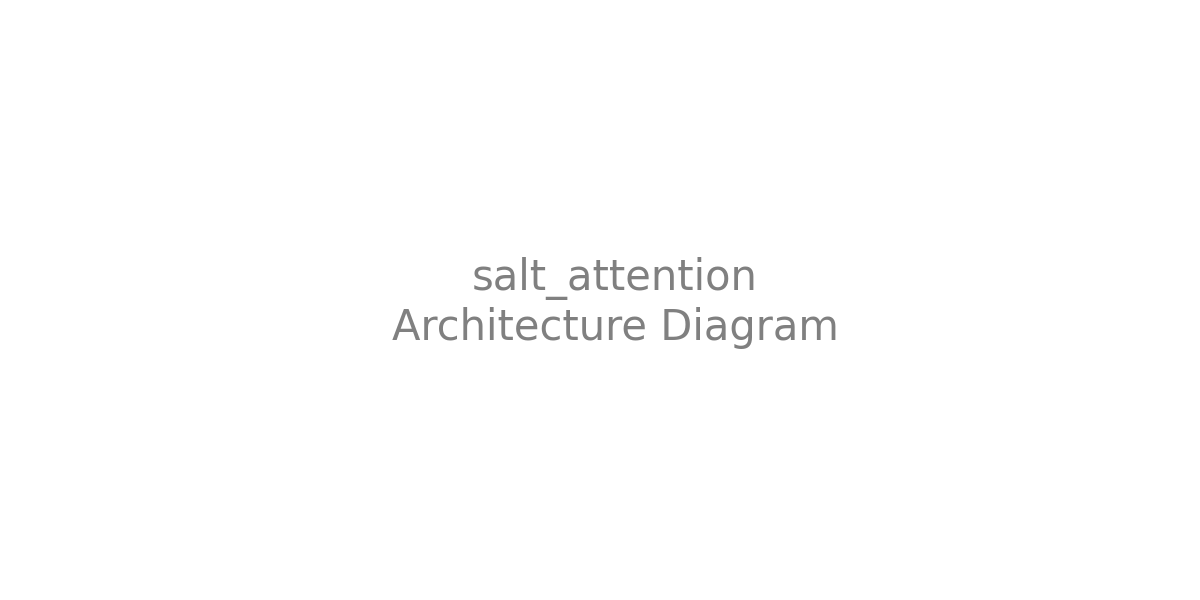
\includegraphics[width=\linewidth]{figures/architecture.png}
\caption{High-level architectural diagram of salt.}
\label{fig:arch\_salt}
\end{figure}

